% 二维随机变量
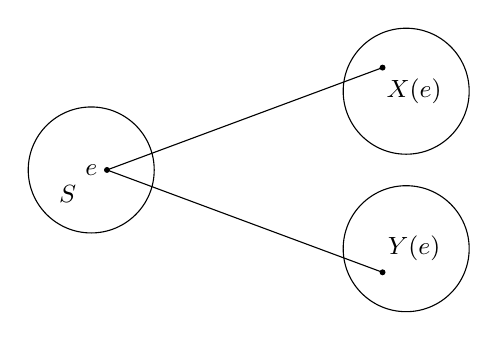
\begin{tikzpicture}
  % S = {e}
  \draw (0,0) circle [radius=0.8];
  \node at (0,0) {\small $e$};
  \node at (-0.3,-0.3) {\small $S$};

  % X = X(e)
  \draw (4,1) circle [radius=0.8];
  \node at (4.1,1) {\small $X(e)$};

  % Y = Y(e)
  \draw (4,-1) circle [radius=0.8];
  \node at (4.1,-1) {\small $Y(e)$};

  % 端点
  \draw [fill] (0.2,0) circle [radius=0.03];
  \draw [fill] (3.7,1.3) circle [radius=0.03];
  \draw [fill] (3.7,-1.3) circle [radius=0.03];
  % 连线
  \draw [thin] (0.2,0) -- (3.7,1.3);
  \draw [thin] (0.2,0) -- (3.7,-1.3);

\end{tikzpicture}
